\subsection{デジタル入力装置}
\subsubsection{ボタン}\label{button}
\begin{table}[H]
  \begin{widerrows}
    \begin{tabular}{|p{\colF}|p{\colG}|}	\hline
    名称 & ボタン(ぼたん)\\ \hline
    接続箇所 & デジタルコネクタ (3pin)\\ \hline
    機能概要 & ボタンが押されているか、押されていないかを調べる\\ \hline
    \end{tabular}
  \end{widerrows} 
\end{table}

\begin{table}[H]
  \begin{widerrows}
    \begin{tabular}{|p{\colF}|p{\colG}|}	\hline
    サンプルコードの場所 & 05/digin.hsp\\ \hline
    raspiへの入力 & ボタンが押されていると1、押されていないと0の値になる。\\ \hline
    raspiへの入力方法 & val = gpioin(GPIO番号)\\ \hline
    raspiからの出力 & なし\\ \hline
    raspiからの出力方法 & なし\\ \hline
    \end{tabular}
  \end{widerrows} 
\end{table}

\begin{table}[H]
  \begin{widerrows}
    \begin{tabular}{|p{\colF}|p{\colG}|} \hline
    使い道 & ゲームのコントローラーのボタン\\ \hline
    注意事項 & 強く押して壊さないように注意\\ \hline
    補足 & ボタンを押すことによって、中に入っている\ruby{金属}{きん|ぞく}が\ruby{繋}{つな}がり電気が流れます。\\ \hline
    \end{tabular}
  \end{widerrows} 
\end{table}

\begin{figure}[H]
  \begin{widerrows}
    \begin{tabular}{|p{\colH}|p{\colI}|p{\colH}|p{\colI}|} \hline
    外観 & 
    \begin{minipage}[t]{\linewidth}
      \smallskip
        \centering
        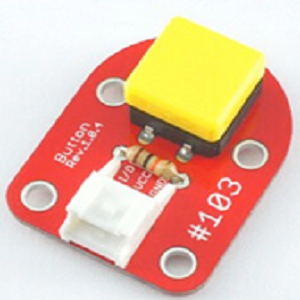
\includegraphics[width=0.5\linewidth]{images/chap05/text05-img028.png}
        \caption{ボタン}
        \smallskip
      \end{minipage} &
      回路記号 & 
      \begin{minipage}[t]{\linewidth}
      \smallskip
        \centering
        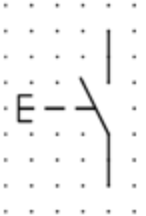
\includegraphics[width=0.3\linewidth]{images/chap05/text05-img045.png}
        \caption{ボタンの回路図}
        \smallskip
      \end{minipage}\\ \hline
    \end{tabular}
  \end{widerrows} 
\end{figure}
